%!TEX root=../../sbc-template.tex

Os dados experimentais utilizados no escopo desse trabalho são oriundos de uma base de dados pública do Hospital Universitário Chittagong em Bangladesh com $150$ pacientes e $1830$ imagens de lâminas de sangue \cite{Yang:2020}, capturadas por uma câmera de celular conectada a um microscópio. As imagens obtidas possuem a resolução de $\SI[parse-numbers=false]{4032 \times 3024}{\pixel}$ e, para cada uma, existe um arquivo com os rótulos contendo informações dos tamanhos circulares e localizações dos protozoários da malária ou das células brancas do sangue. As anotações relativas às células brancas foram descartadas por não serem do escopo de interesse do problema em questão. No total, havia $\num{84509}$ rótulos para a classe de interesse nos exemplos da base de dados.

Como os modelos da Família YOLO utilizam caixas retangulares para detecção dos objetos, foi necessário realizar uma etapa de pré-processamento para substituir os círculos originalmente disponíveis. Para tanto, calculou-se o raio do círculo e obteve-se entãoo a caixa delimitadora de formato quadrado circunscrita ao círculo, conforme exemplificado na Figura \ref{fig:example-class}.  Ademais, observou-se que $\SI{0.55}{\percent}$ das imagens não possuíam rótulos.

 \begin{figure}[h!]
 	\centering
 	\hfill \subfloat[Imagem sem rótulos]{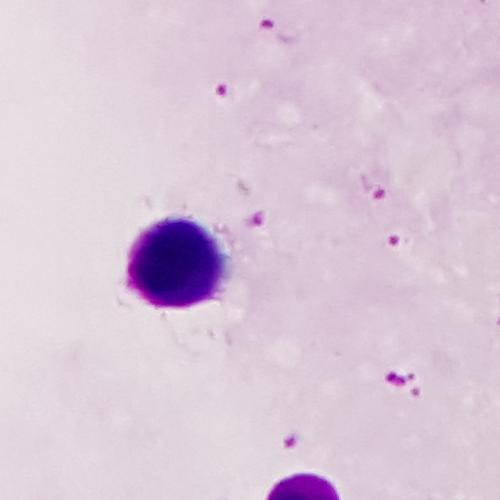
\includegraphics[width=0.32\linewidth]{img/sample/blood-raw.jpg}}
 	\hfill \subfloat[Centroides]{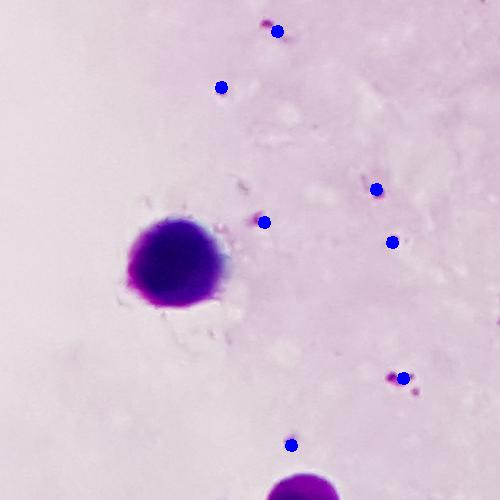
\includegraphics[width=0.32\linewidth]{img/sample/blood-centers.jpg}}
 	\hfill \subfloat[Centroides e caixa delimitadora]{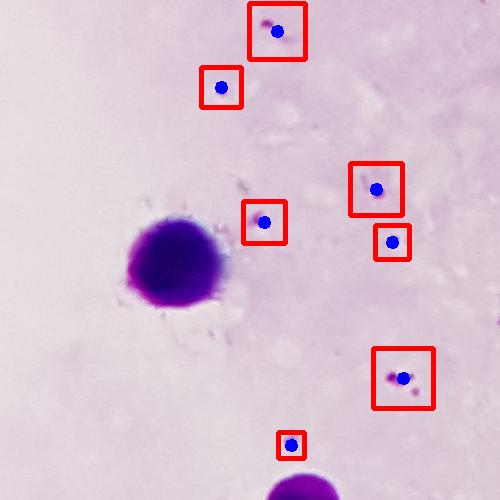
\includegraphics[width=0.32\linewidth]{img/sample/blood-squares.jpg}}
 	\caption{Exemplo com a imagem original, acrescida de centroides e das caixas delimitadoras quadradas.}
 	\label{fig:example-class}
\end{figure}

Ao efetuar uma análise exploratória das imagens e dos rótulos disponíveis nas mesmas, conforme histograma da Figura \ref{fig:histogram}, foi possível perceber que a maioria das imagens ($967$) possuía até $25$ caixas delimitadoras. Do total de imagens,  somente $17$ não possuíam nenhum rótulo ($\SI{0.55}{\percent}$ dos exemplos da base de dados), indicando pacientes saudáveis. Embora não sejam relevantes para o aprendizado de padrões a respeito dos protozoários, colaboram no aprendizado do \emph{background} pelos modelos de detecção com \emph{Deep Learning}. Observou-se também que poucas imagens possuíam mais de $200$ protozoários com caixas delimitadoras, correspondendo a $\SI{2.1}{\percent}$ dos exemplos da base de dados.

 \begin{figure}[ht]
    \centering
    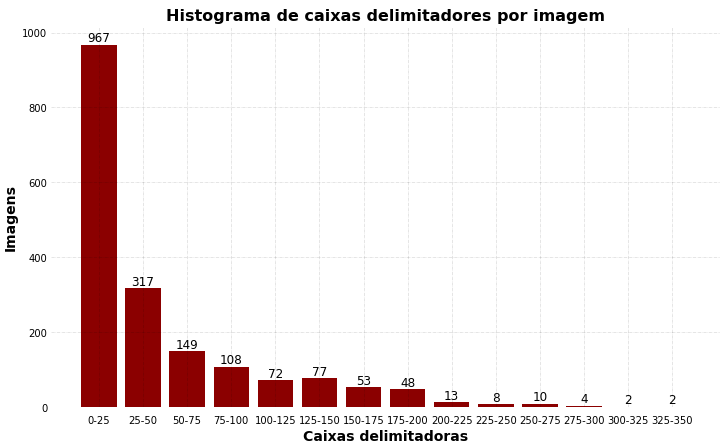
\includegraphics[width=0.9\textwidth]{img/histogram.png}\hfill
    \caption{Histograma da quantidade de caixas delimitadoras por imagens da base de dados.}
    \label{fig:histogram}
\end{figure}

Um mapa de calor foi elaborado para ilustrar a disposição espacial dos rótulos das caixas delimitadoras nas imagens da base de dados, conforme mostrado na Figura \ref{fig:heat-map}. Nota-se uma distribuição uniforme de tais caixas sobre toda a região visível pelo microscópio, o que reforça a dificuldade na tarefa de detecção por não haver boas regiões candidatas na distribuição \emph{a priori} dos exemplos.

\begin{figure}[H]
    \centering
    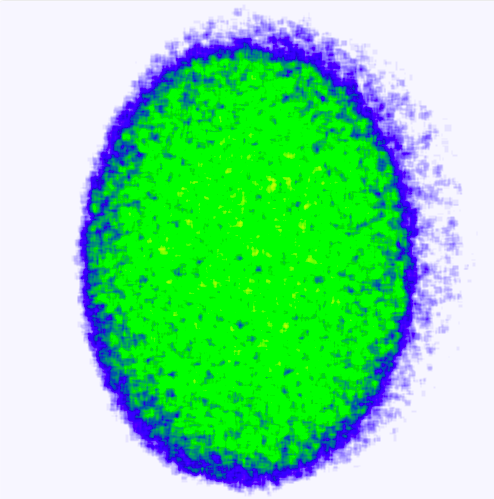
\includegraphics[width=0.7\textwidth,height=0.525\textwidth]{img/heat-map.png}\hfill
    \caption{Mapa de calor da disposição das caixas delimitadoras nos exemplos.}
    \label{fig:heat-map}
\end{figure}

Analisando o tamanho das caixas delimitadores, conforme disposto na Tabela \ref{tab:bounding-boxes}, é possível afirmar que sua área é de cerca de $\SI{1.5}{\percent}$ da área total da imagem. Para a detecção de objetos com R-CNNs da família YOLO, em particular, objetos com percentual menor que $\SI{12.5}{\percent}$ da área total são considerados de difícil detecção \cite{Xiao:2021}. Esse fato reforça as dificuldades em abordar um problema realístico no âmbito da detecção automática de objetos

\begin{table}[h!]
\begin{center}
\caption{Descrição estatística do tamanho das caixas delimitadoras.} 
\begin{footnotesize}
\begin{tabular}{cccccccccccc}
\toprule
        & \multicolumn{3}{c}{\textbf{Lado}} & & \multicolumn{3}{c}{\textbf{Caixas Delimitadoras}} \\
        \cmidrule{2-4} \cmidrule{6-8}
      &  \textbf{Média} & \textbf{Máx} & \textbf{Mín} & &     \textbf{Média} & \textbf{Máx} & \textbf{Mín}\\
\midrule
\label{tab:bounding-boxes}
\textbf{Protozoário} & $41.84 \pm 9.71$ & $191$ & $3$ & & $46.17 \pm 56.35$ & $341$ & $0$\\
\bottomrule
\end{tabular}
\end{footnotesize}
\end{center}
\end{table}